\documentclass[notes, xcolor = dvipsnames]{beamer}

\usetheme{Warsaw}

\usepackage{amsmath}
\usepackage{graphicx}

\title{Memory Barriers: A Hardware view for Software Hackers}
\subtitle{Paul E. McKenney}

\author{Presented by \\ Akshay Gopalakrishnan}

\begin{document}
  
    \begin{frame}
        
        \maketitle
    \end{frame}


    \begin{frame}{Introduction}
        
        \begin{itemize}
            \item This paper represents the inner working of hardware that results in several non-sequential behaviors of our concurrent programs
            \item The paper is rife with examples as well as showcasing the reasons for having such hardware features which in turn help in our programs performing better.
            \item Along with the positives the author also carefully cautions why such rampant changes for performance might result in highly non-trivial behaviors being showcased by the hardware running our programs.
            \item The paper concludes by discussing the then versions of several concurrent hardware that exhibit different non-sequential behaviors.
        \end{itemize}

    \end{frame}

    \begin{frame}{Cache structures}
        
        \begin{figure}
            \makebox[\textwidth][c]{
                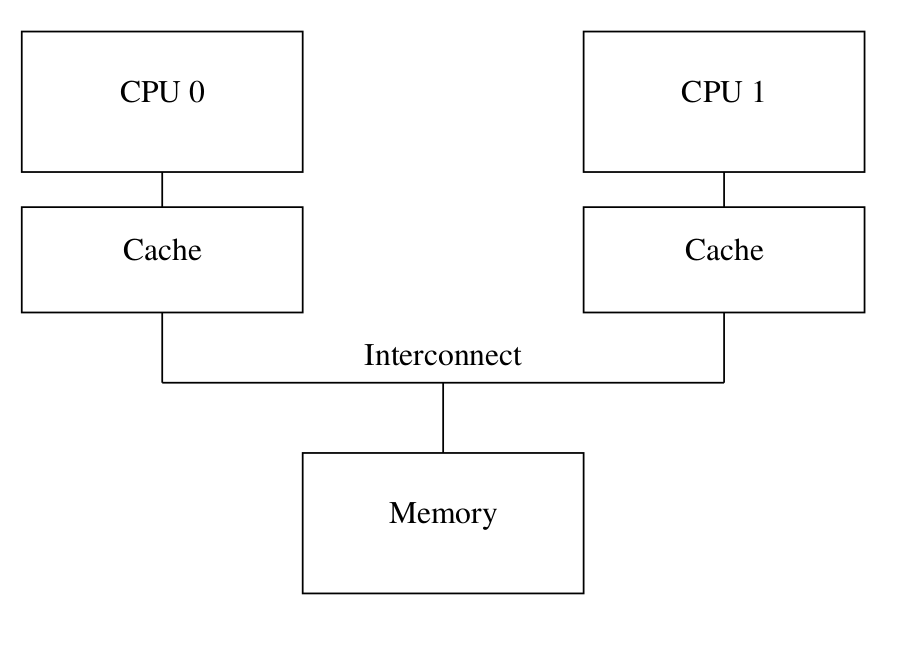
\includegraphics[scale=0.6]{CacheStructure.png}
            }
        \end{figure}

        \begin{itemize}
            \item An extra chunk of memory local to a given cpu (or multiple cpus in bigger systems).
            \item Data read from memory will also be saved in the cache if there is space. 
            \item Any subsequent accesses to the same memory will be first looked at in the cache and if not present, from the main memory.
        \end{itemize}

    \end{frame}

    \begin{frame}{The usefullness of Caches}
        
        \begin{itemize}
            \item Used for faster access of memory. 
            \item Useful when a single shared memory location is being accessed several times but not changed. 
            \item Need to read from main memory which is at least 10x times slower than accessing caches.
            \item Overall performance of program is significantly improved. 
        \end{itemize}

    \end{frame}

    \note{
        In modern systems there are multiple cache levels that exist, each of which is based on the scope. 
        For instance, L1 cache is local to just one core. Whereas L2 is to multiple cores in the same processor (could also be others). 
        All this layering is done for performance, part of the reason why we have such highly non-trivial behaviors of our concurrent programs.
    }

    \begin{frame}{THe MESI protocol}
        
        \begin{itemize}
            \item Multiple caches need to be in synchronization to ensure no stale data in caches exist. 
            \item Caches can communicate with each other via the interconnect network.
            \item We require a protocol to ensure that caches lines are updated accordingly. 
        \end{itemize}

        An example of such a protocol is MESI (Modified Exclusive Shared and Invalid).
        \begin{itemize}
            \item Modified - cache line has the upto date data which resides in memory and the data has been stored by the corresponding CPU. 
            \item Exclusive - cache line is not updated with the recent memory store done by the corresponding CPU. 
            \item Shared  - cache line is in read-only state (CPU needs to consult with other CPU caches before being able to write to it)
            \item Invalid - "empty" cache line and new data can be put here. 
        \end{itemize}


    \end{frame}

    \note{
        Modified state is when my CPU is writiing to memory some data as well as duly updated the cache line. Now this line has the only copy of the latest data in memory. 
        Exlcusive is one step behind modified state, wherein the CPU has updated memory, but not just its cache line. 
        Shared state is when more than one cache line has the same data of memory. This only means, if I want to change one cache line, I must inform the others too. 
        Invalid state can contain any stale data that is never going to be read by the CPU (as it is stale).
    }

    \begin{frame}{Example of Cache Communication methods}
        
    \end{frame}

    \begin{frame}{Example}
        
    \end{frame}

    \begin{frame}{Need for Write Buffers}
        
    \end{frame}

    \begin{frame}{Added Complications}
        
    \end{frame}

    \begin{frame}{Example}

    \end{frame}

    \begin{frame}{Here comes Write Memory Barriers}
        
    \end{frame}

    \begin{frame}{Need for Invalidate Queues}
        
    \end{frame}

    \begin{frame}{Added Complications}
        
    \end{frame}

    \begin{frame}{Example}
        
    \end{frame}

    \begin{frame}{Here comes Read Memory Barriers}
        
    \end{frame}

    \begin{frame}{Barrier instructions offered by Linux}
        
    \end{frame}

    \begin{frame}{Hardware Example: Alfa}
        
    \end{frame}

    \begin{frame}{Hardware Example: x86}
    
    \end{frame}

    \begin{frame}{Conclusion}
        
    \end{frame}

\end{document}